\documentclass[indonesian,12pt]{report}

\usepackage{fontspec}
\usepackage[provide=*]{babel}
\usepackage[a4paper, margin=3cm]{geometry}
\usepackage{setspace}
\usepackage{graphicx}
\usepackage{array}
\usepackage{tikz}

\usepackage{listings}
\usepackage{xcolor}

\setmainfont{Times New Roman}
\renewcommand{\baselinestretch}{1.5}
\renewcommand{\thesection}{\Alph{section}}
\renewcommand{\thesubsection}{\arabic{subsection}.}
\renewcommand{\thesubsubsection}{\arabic{subsection}.\arabic{subsubsection}.}
\setcounter{secnumdepth}{3}

\usetikzlibrary{shapes.geometric, shapes.symbols, arrows.meta, positioning, calc}

\begin{document}

\begin{titlepage}
    \centering

    \textbf{
    LAPORAN PRAKTIKUM\\
    PRAKTIKUM PEMROGRAMAN KOMPUTER DASAR\\
    PERTEMUAN X\\
	X
    }

    \vspace{2cm}

    
\includegraphics[width=0.4\textwidth]{images/logo.png}

    \vspace{3cm}

    Disusun Oleh:

    \vspace{0.2cm}

    \begin{tabular}{p{4cm} c l}
        Nama            & : & John Doe \\
        NIM             & : & 123456789 \\
        Kelas           & : & A2 \\
        Dosen Pengampu  & : & Jane Smith
    \end{tabular}

    \vfill

    \textbf{
    PROGRAM STUDI D-IV TEKNOLOGI REKAYASA PERANGKAT LUNAK\\
    DEPARTEMEN TEKNIK ELEKTRO DAN INFORMATIKA\\
    SEKOLAH VOKASI\\
    UNIVERSITAS GADJAH MADA\\
    YOGYAKARTA\\
    2026
    }

\end{titlepage}

\begin{newpage}
    \section{Quiz}
        \subsection{Score Calculator}
        \subsubsection{Flowchart}:

        \vspace{0.5cm}

        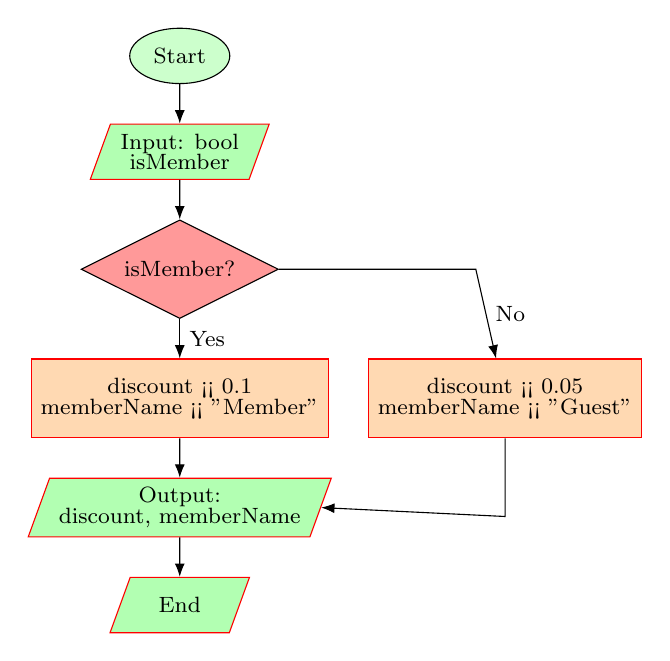
\begin{tikzpicture}[
            node distance=0.5cm and 0.5cm,
            flowtext/.style={
                align=center,
                font=\fontsize{8pt}{5pt}\selectfont,
            },
            oval/.style={
                ellipse,
                draw,
                fill=green!20,
                minimum height=2em,
                flowtext
            },
            diam/.style={
                diamond,
                aspect=2,
                draw,
                fill=red!40,
                flowtext
            },
            block/.style={
                rectangle,
                draw,
                fill=blue!20,
                rounded corners,
                text width=3cm,
                minimum height=2em,
                flowtext
            },
            trap/.style={
                trapezium,
                trapezium left angle=70,
                trapezium right angle=110,
                draw=red,
                fill=green!30,
                minimum height=2em,
                flowtext
            },
            rect/.style={
                rectangle,
                draw=red,
                fill=orange!30,
                minimum height=1cm,
                flowtext
            },
            offpage/.style={
                signal,
                signal to=south,
                draw,
                fill=yellow!30,
                text width=3cm,
                minimum height=1cm,
                flowtext,
            },
            line/.style={
                draw,
                font=\fontsize{8pt}{5pt}\selectfont,
                -{Latex}
            }
        ]

            \node [oval] (start) {Start} ;
            \node [trap, below=of start] (input-1) {Input: bool\\isMember};
            \node [diam, below=of input-1] (decision-1) {isMember?};
            \node [rect, below=of decision-1] (process-1) {discount << 0.1\\memberName << "Member"};
            \node [rect, right=of process-1] (process-2) {discount << 0.05\\memberName << "Guest"};
            \node [trap, below=of process-1] (output-1) {Output: \\discount, memberName};
            \node [trap, below=of output-1] (end) {End};

            \path [line] (start) -- (input-1);
            \path [line] (input-1) -- (decision-1);
            \path [line] (decision-1) -- node [right] {Yes} (process-1);
            \path [line] (decision-1.east) -- ++(2.5,0) -- node [right] {No} (process-2);
            \path [line] (process-1) -- (output-1);
            \path [line] (process-2) -- ++(0,-1.5) -- (output-1.east);
            \path [line] (output-1) -- (end);
        \end{tikzpicture}

    \lstset{
        language=C++,
        commentstyle=\slshape,
        basicstyle=\ttfamily\fontsize{8pt}{5pt}\selectfont,
        numbers=left,
        numberstyle=\tiny,
        frame=single,
        breaklines=true,
        showstringspaces=false,
        tabsize=2,
        moredelim={**[is][\hlblock\slshape]{[[}{]]}}
    }
    \subsubsection{Source Code}
\begin{lstlisting}
#include <iostream>
using namespace std;

void fibonacciSequence(int limit, int a = 0, int b = 1){
    if(limit == 0) return;
    cout << a;
    if(limit != 1) cout << ", ";
    fibonacciSequence(limit - 1, b, a + b);
}

int main(){
    int limit;
    cout << "Input limit: ";
    cin >> limit;
    cout << "Fibonacci Sequence: ";
    fibonacciSequence(limit);
}
\end{lstlisting}
	\subsubsection{Output}

	\vspace{0.2cm}
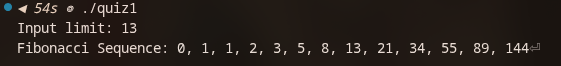
\includegraphics[width=1\textwidth]{images/quiz1.png}\\
	\subsubsection{Penjelasan}

	Fungsi \texttt{fibonacciSequence} digunakan untuk menampilkan deret Fibonacci dengan pendekatan rekursif. Fungsi ini menerima parameter \texttt{limit} sebagai jumlah bilangan yang akan ditampilkan, serta parameter \texttt{a} dan \texttt{b} sebagai dua bilangan awal deret. Jika nilai \texttt{limit} sama dengan 0, fungsi berhenti sebagai kondisi dasar. Jika belum, fungsi mencetak nilai \texttt{a}, kemudian memanggil dirinya sendiri dengan nilai \texttt{b} dan hasil penjumlahan \texttt{a + b}. Fungsi \texttt{main} menerima input batas deret dari pengguna, kemudian memanggil fungsi tersebut untuk menampilkan deret Fibonacci.

\end{newpage}
\end{document}